\documentclass[11pt]{article}
\usepackage[english]{babel}
\usepackage{amsmath,amssymb,amsfonts}
\usepackage{fullpage}
\usepackage{hyperref}
\usepackage{float}
\usepackage{xcolor}
\usepackage{booktabs}
\usepackage{graphicx}
\usepackage{listings}
\usepackage{titlesec}
% Disable paragraph indentation
\setlength{\parindent}{0pt}%
\setlength{\parskip}{\baselineskip}%
\titleformat{\section}{\large\bfseries}{\thesection}{1em}{}

\lstset{
  language=Python,                 % Set language to Python
  basicstyle=\ttfamily\footnotesize, % Set font and size
  keywordstyle=\color{blue},       % Keywords in blue
  stringstyle=\color{red},         % Strings in red
  commentstyle=\color{green!50!black}, % Comments in green
  backgroundcolor=\color{yellow!10}, % Light gray background
  frame=single,                    % Frame around the code
  numbers=left,                    % Line numbers on the left
  numberstyle=\tiny\color{gray},   % Style for line numbers
  tabsize=5,                       % Set tab width
  showstringspaces=false,           % Hide whitespace symbols
  captionpos=b                     % Caption at the bottom
}

\begin{document}
\title{Assignment2 - DD2424}
\author{Silpa Soni Nallacheruvu}
\date{}
\maketitle

\section*{Gradient Check}

To verify the correctness of my analytical gradients for the two-layer neural network, I implemented a gradient comparison against numerically computed gradients from PyTorch. The gradients were derived as follows:

\[
\frac{\partial \mathcal{L}}{\partial W^{[2]}} = \frac{1}{n} (P - Y) H^\top + 2\lambda W^{[2]}, \quad 
\frac{\partial \mathcal{L}}{\partial b^{[2]}} = \frac{1}{n} \sum_{i=1}^{n} (P - Y)_i
\]

\[
\frac{\partial \mathcal{L}}{\partial W^{[1]}} = \frac{1}{n} (G \circ \mathbf{1}_{H > 0}) X^\top + 2\lambda W^{[1]}, \quad 
\frac{\partial \mathcal{L}}{\partial b^{[1]}} = \frac{1}{n} \sum_{i=1}^{n} (G \circ \mathbf{1}_{H > 0})_i
\]

The implementation was tested using a small synthetic input and compared layer-wise with PyTorch-generated gradients. The results were:

\begin{lstlisting}[caption={Relative error of analytical and numerical gradients}, label={lst:gradients}]
Relative errors in W:
Layer 0: max relative error = 1.63e-14
Layer 1: max relative error = 2.12e-16

Relative errors in b:
Layer 0: max relative error = 1.60e-15
Layer 1: max relative error = 3.08e-16
\end{lstlisting}

The extremely small relative errors confirm that the analytical gradients are implemented correctly and align closely with the numerical gradients. 
\section*{Cyclical Learning Rate Training Curves}

\subsection*{Exercise 3}
The curves below illustrate the training and validation cost, loss, and accuracy using this learning rate schedule using the default values for the hyper-parameters from the assignment.

\begin{figure}[H]
    \centering
    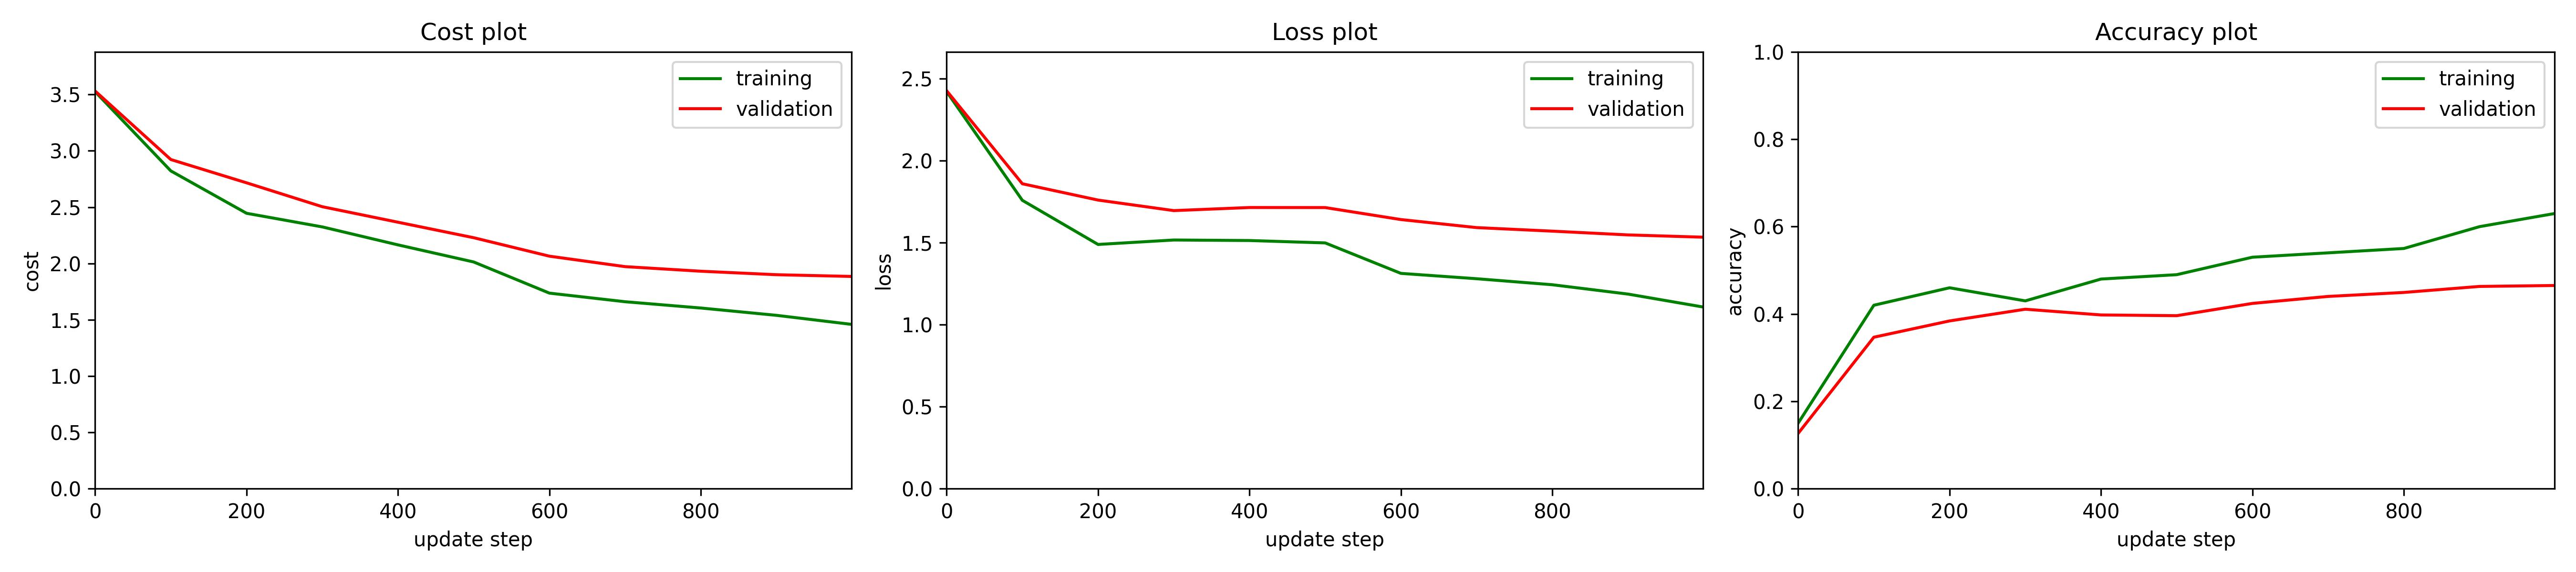
\includegraphics[width=1\textwidth]{cyclic_training_curves_ex3.jpg}
    \caption{Training curves (cost, loss and accuracy) for one cycle of training.}
    \label{fig:cyclical_lr_curves1}
\end{figure}


The following are accuracy results: 
\begin{lstlisting}[caption={Training and validation accuracy for one cycle}, label={lst:accuracy}]
Accuracy for training : 64.56% with steps 1000
Accuracy for validation : 46.52% with steps 1000
Accuracy for testing : 47.54% with steps 1000
\end{lstlisting}

As seen in the plots, the training and validation curves in \autoref{fig:cyclical_lr_curves1} show consistent descent, that resemble \texttt{Figure 3} in the assignment.
The curves are smooth and reflect the expected rise and fall of learning rate across one cycle. 

The cycle length was set to 1000 iterations, with a minimum learning rate of \(1e^{-5}\) and a maximum learning rate of \(1e^{-1}\) as seen in the plot below.
\begin{figure}[H]
    \centering
    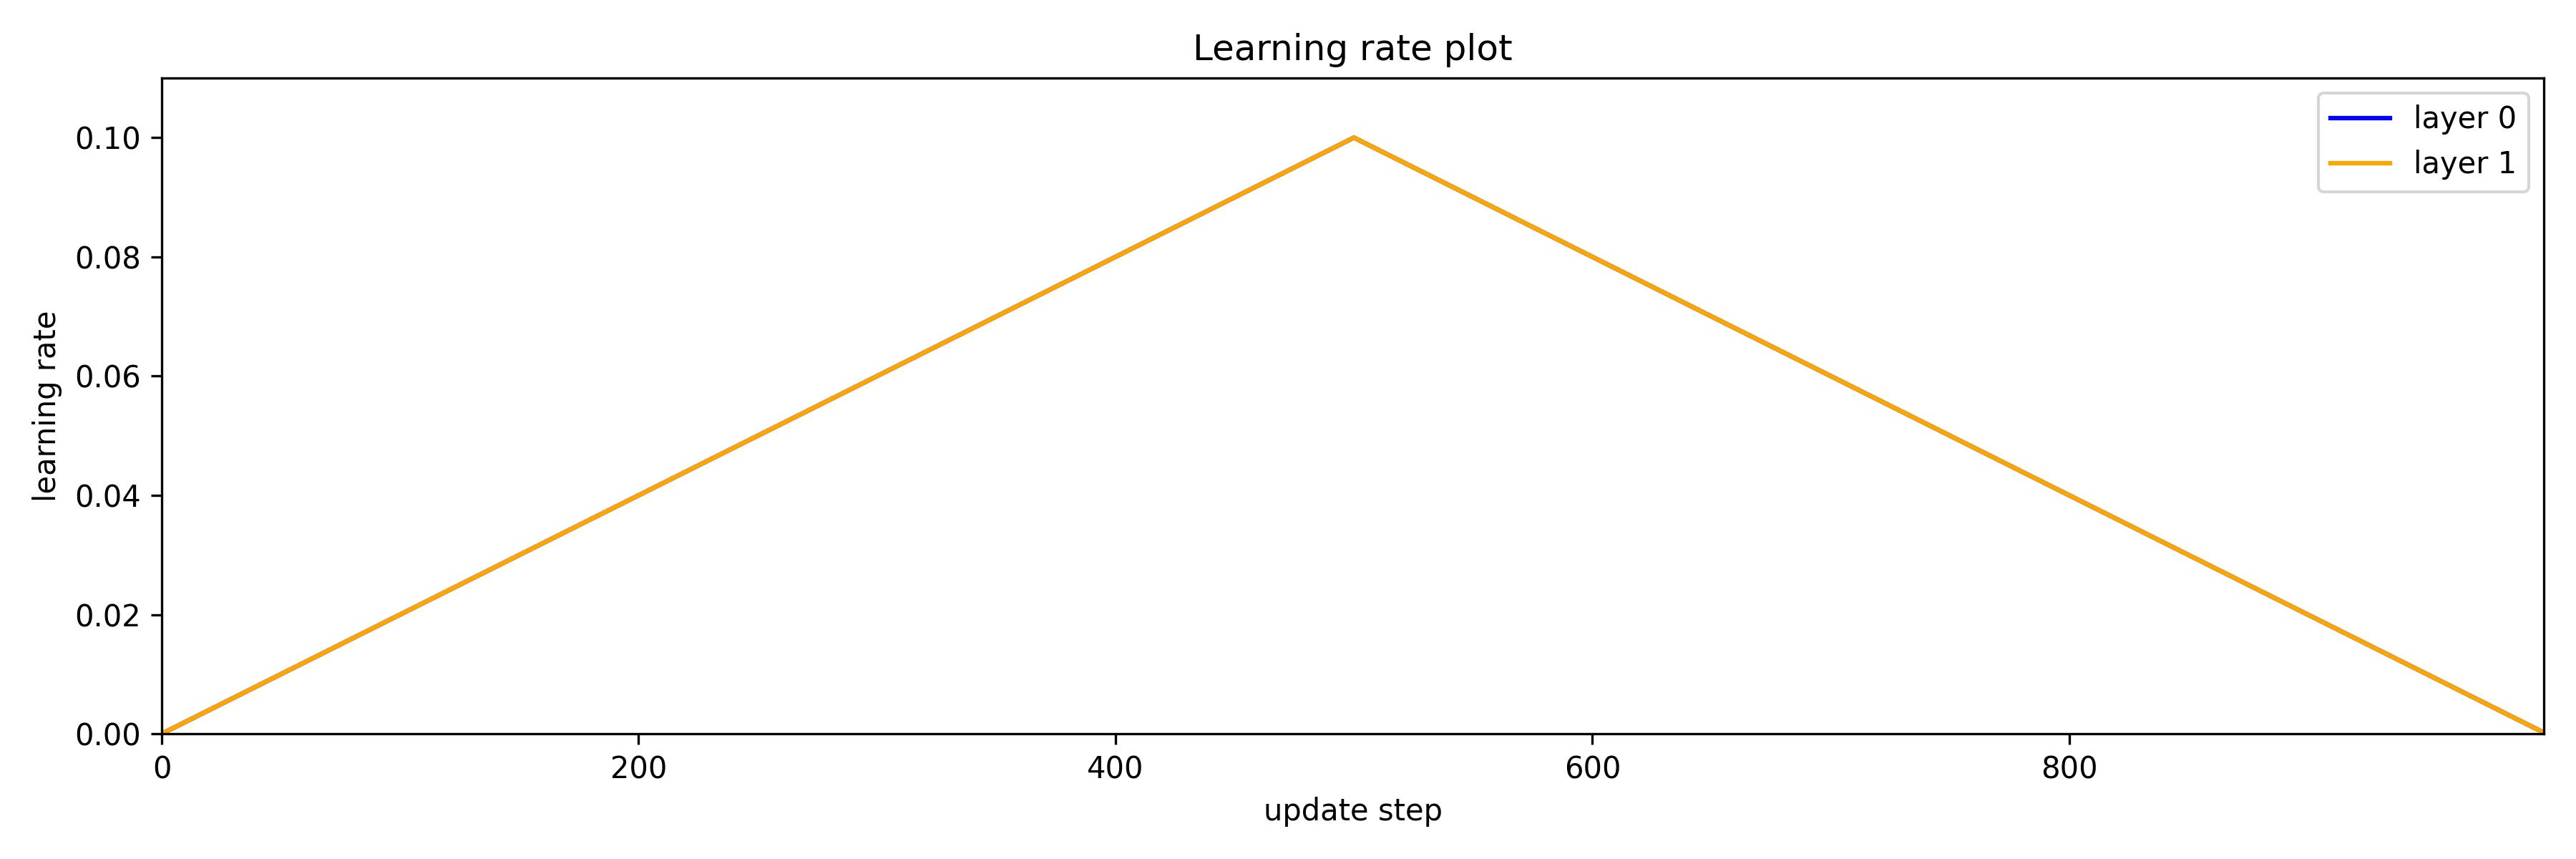
\includegraphics[width=0.8\textwidth]{cyclic_eta1.jpg}
    \caption{Plot of learning rate across the update steps.}
    \label{fig:cyclic_eta1}
\end{figure}


\subsection*{Exercise 4}

The same training was performed with a longer cycle length of 4800 iterations, while keeping the minimum and maximum learning rates the same as before.
The following are the training and validation curves for this run:
\begin{figure}[H]
    \centering
    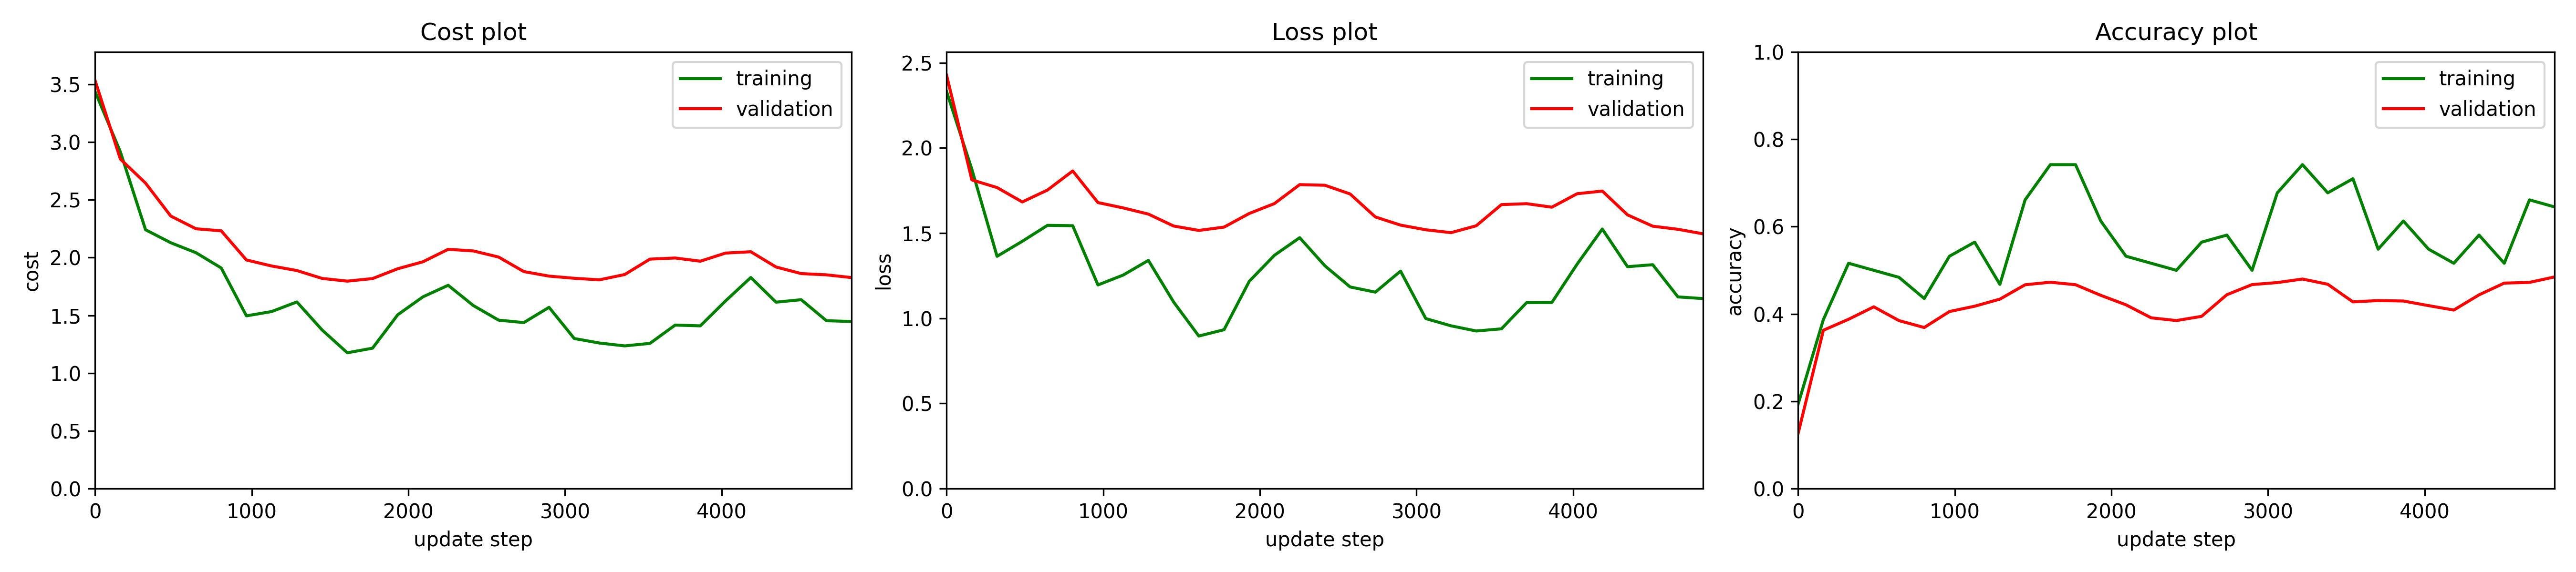
\includegraphics[width=1\textwidth]{cyclic_training_curves_ex4.jpg}
    \caption{Training curves (cost, loss and accuracy) for three cycles of training.}
    \label{fig:cyclical_lr_curves2}
\end{figure}

The following are accuracy results:

\begin{lstlisting}[caption={Training and validation accuracy for three cycles}, label={lst:accuracy2}]
Accuracy for training : 73.90% with steps 4800
Accuracy for validation : 48.54% with steps 4800
Accuracy for testing : 48.81% with steps 4800
\end{lstlisting}

The plot of learning rate across the update steps is shown below:
\begin{figure}[H]
    \centering
    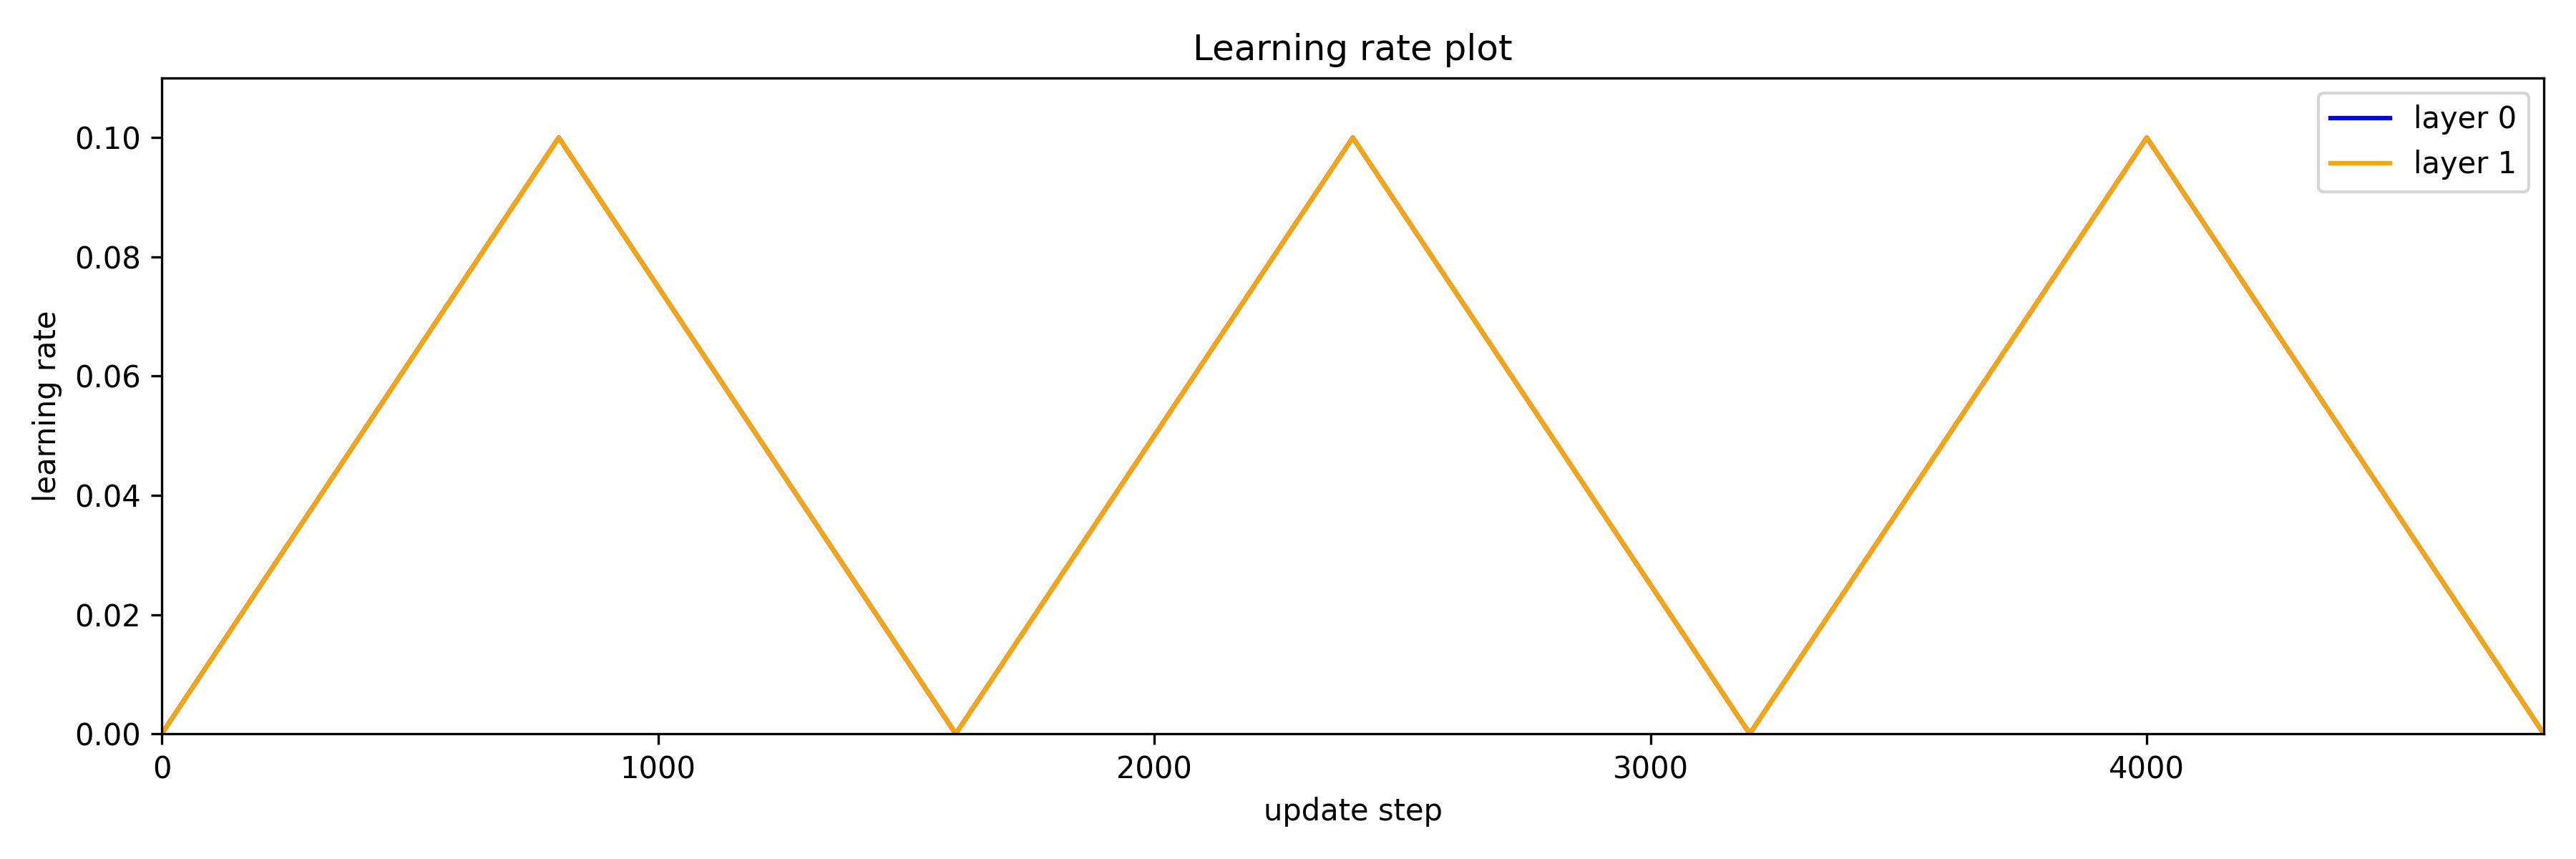
\includegraphics[width=0.8\textwidth]{cyclic_eta2.jpg}
    \caption{Plot of learning rate across the update steps.}
    \label{fig:cyclic_eta2}
\end{figure}

As seen in the plots, the training and validation curves in \autoref{fig:cyclical_lr_curves2} display more fluctuations compared to the first training algorithm, similar to \texttt{Figure 4} in the assignment. 
Despite these oscillations, the validation accuracy improved and converges to a higher value than the first training algorithm.
This suggests that longer cycles help escape local minima and explore the loss landscape more effectively, though at the cost of more training instability.


Overall, cyclical learning rates provided effective control over the optimization dynamics, offering a balance between fast convergence and robustness against overfitting.

\section*{Coarse search for lambda}

I performed a coarse search for lambda by choosing 100 different values of lambda, ranging from $10^{-5}$ to $10^{-1}$ using a uniform grid and logarithm scale as mentioned in the assignment.
I ran the training for one cycle with hyper-parameters set to eta\_min = 1e-5, eta\_max = 1e-1, and n\_batch = 100. 
The training and validation curves for this run are shown below:
\begin{figure}[H]
    \centering
    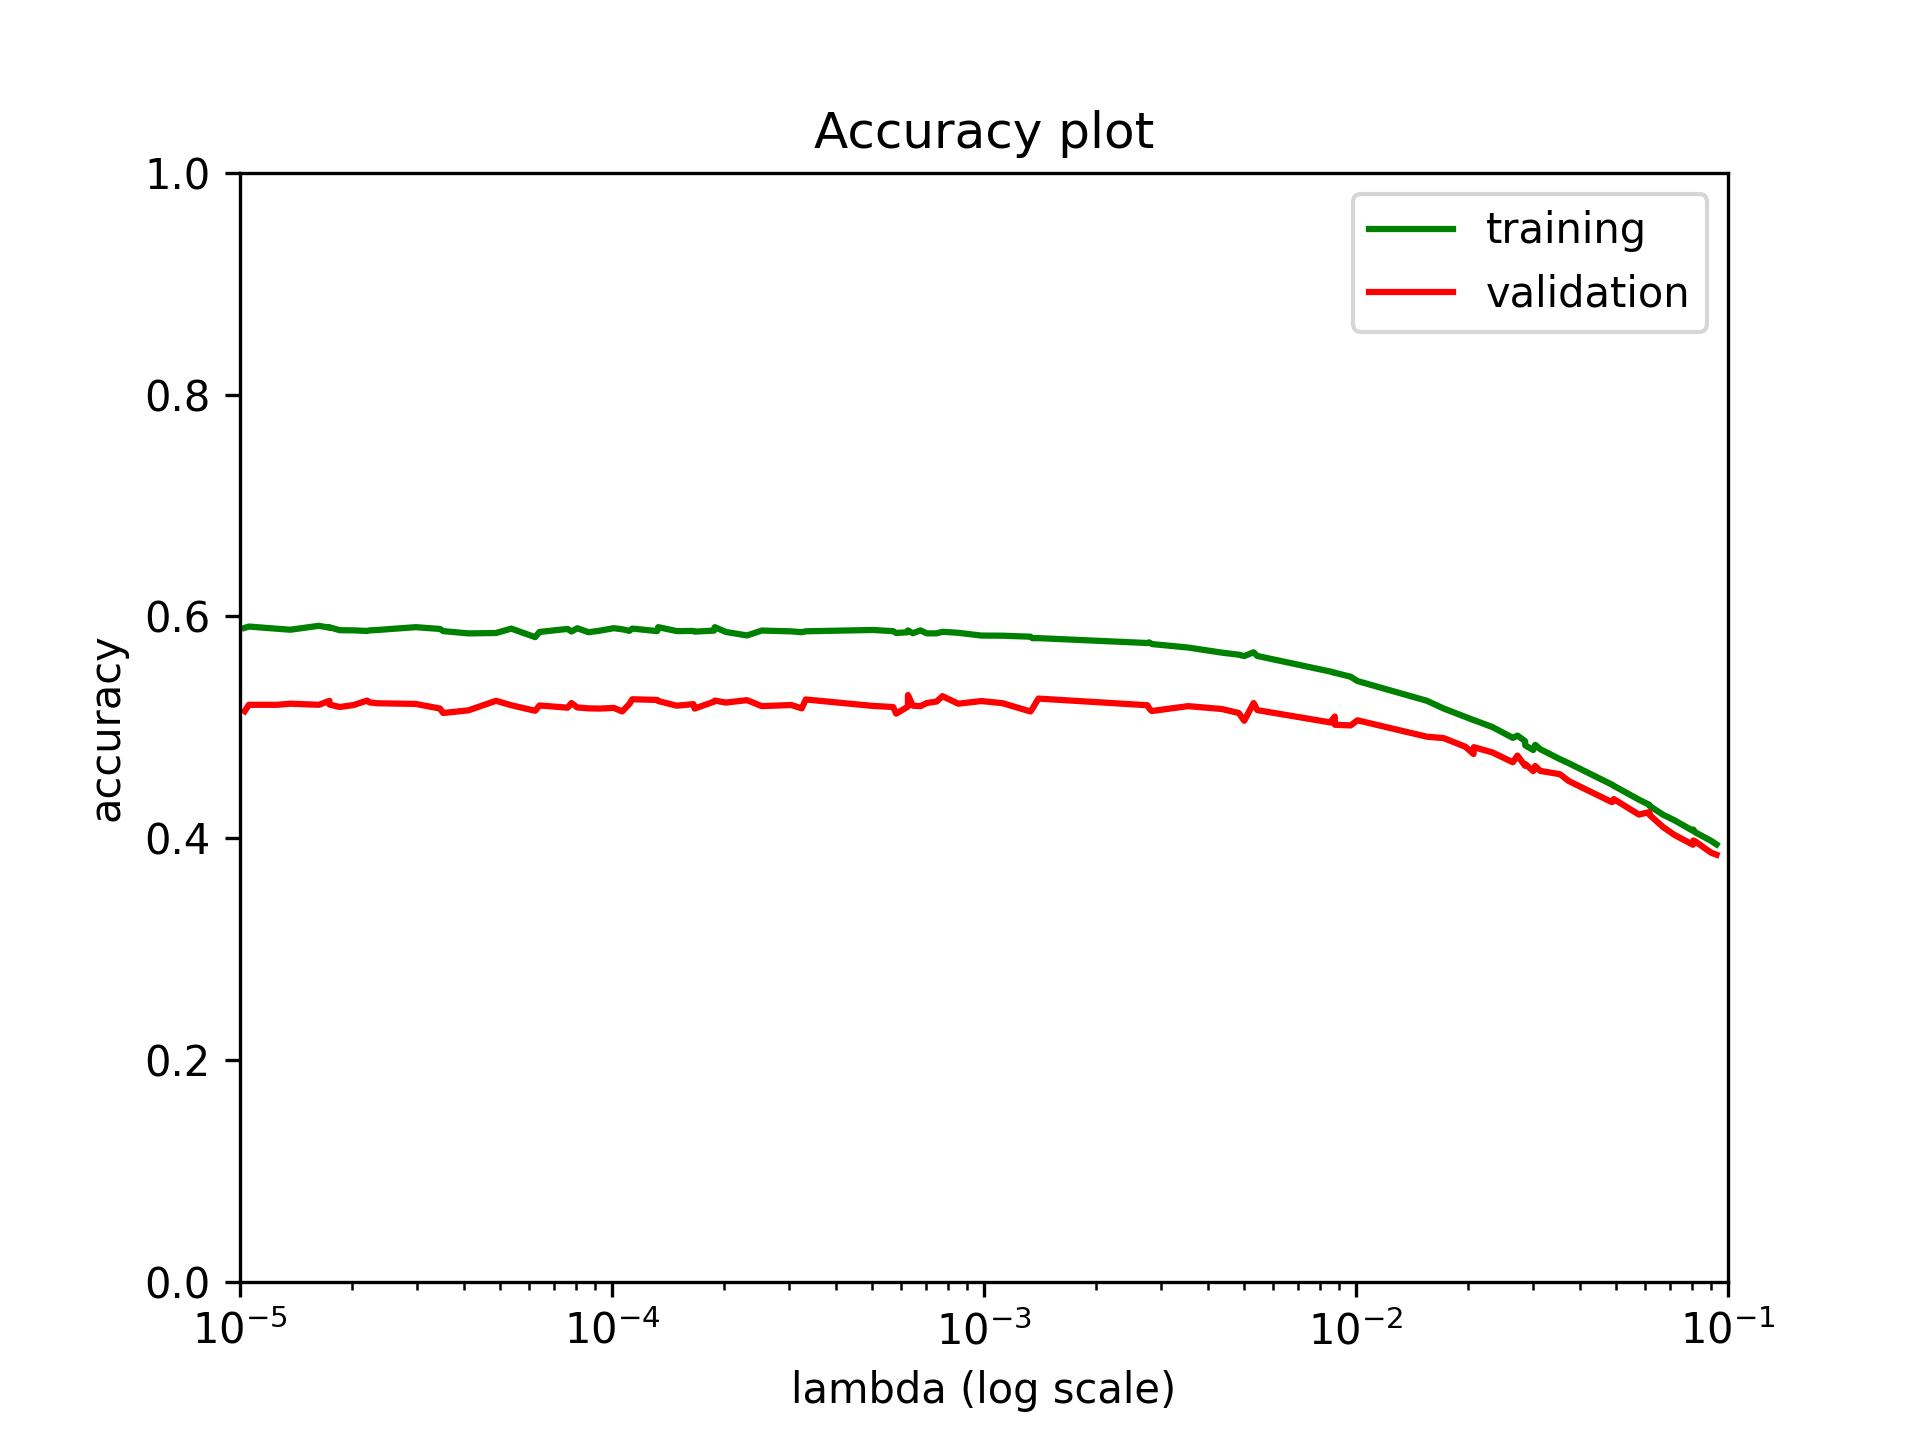
\includegraphics[width=0.8\textwidth]{lambda_accuracies.jpg}
    \caption{Training and validation accuracies for a range of lamdas.}
    \label{fig:coarse_search_curves}
\end{figure}

The following are the best three performing networks based on validation accuracy:
\begin{lstlisting}[caption={Coarse search for lambda}, label={lst:coarse_search}]
lambda=0.0006246592215568911, training accuracy=58.73%, validation accuracy=52.90%
lambda=0.0007730255340781429, training accuracy=58.60%, validation accuracy=52.80%
lambda=0.0014004414195479882, training accuracy=58.03%, validation accuracy=52.58%
\end{lstlisting}

\section*{Fine search for lambda}

I performed a fine search for lambda by choosing 10 different values of lambda in logarithm scale, by shortening the range of lambda to $10^{-4}$ to $10^{-2}$ focusing on the good settings from the coarse search.
I ran the training for two cycles with the same hyper-parameters as before.
The following are the best three performing networks based on validation accuracy:
\begin{lstlisting}[caption={Fine search for lambda}, label={lst:fine_search}]
lambda=0.0022477040596100145, training accuracy=62.12%, validation accuracy=55.12%
lambda=0.004726183203219606, training accuracy=59.92%, validation accuracy=54.50%
lambda=0.0005807904703734551, training accuracy=63.48%, validation accuracy=54.36%
\end{lstlisting}

As mentioned in the assignment, all the 10 values of lambda from the fine search displayed validation accuracies above 50\%, indicating that the model is learning effectively.
The best performing lambda from the fine search was 0.0022, which achieved a training accuracy of 62.12\% and a validation accuracy of 55.12\%.

\section*{Best found lambda}
I performed a final training run with the best lambda value of 0.0022, using the same hyper-parameters as before.
I ran the training for three cycles and excluded 1000 examples from the training set for validation.
The test data was the provided \texttt{test\_batch} dataset. 

The plot below indicates the training and validation curves for this run:
\begin{figure}[H]
    \centering
    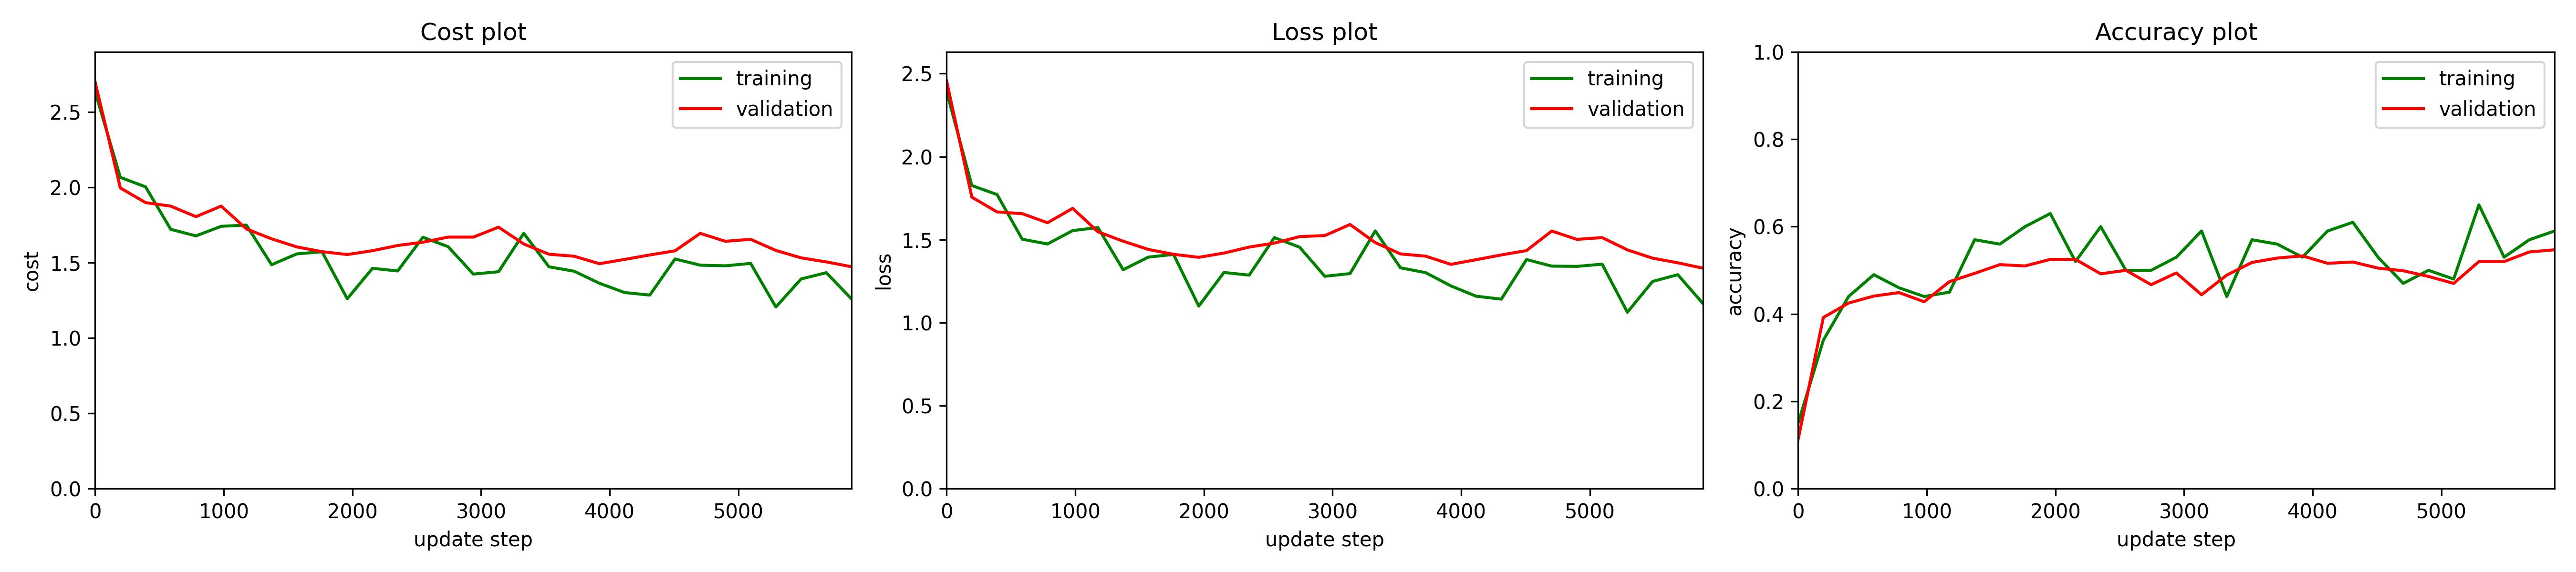
\includegraphics[width=1\textwidth]{cyclic_training_curves_ex5.jpg}
    \caption{Training curves (cost, loss and accuracy) for three cycles of training with best lambda.}
    \label{fig:best_lambda_curves}
\end{figure}

The plot of learning rate across the update steps is shown below:
\begin{figure}[H]
    \centering
    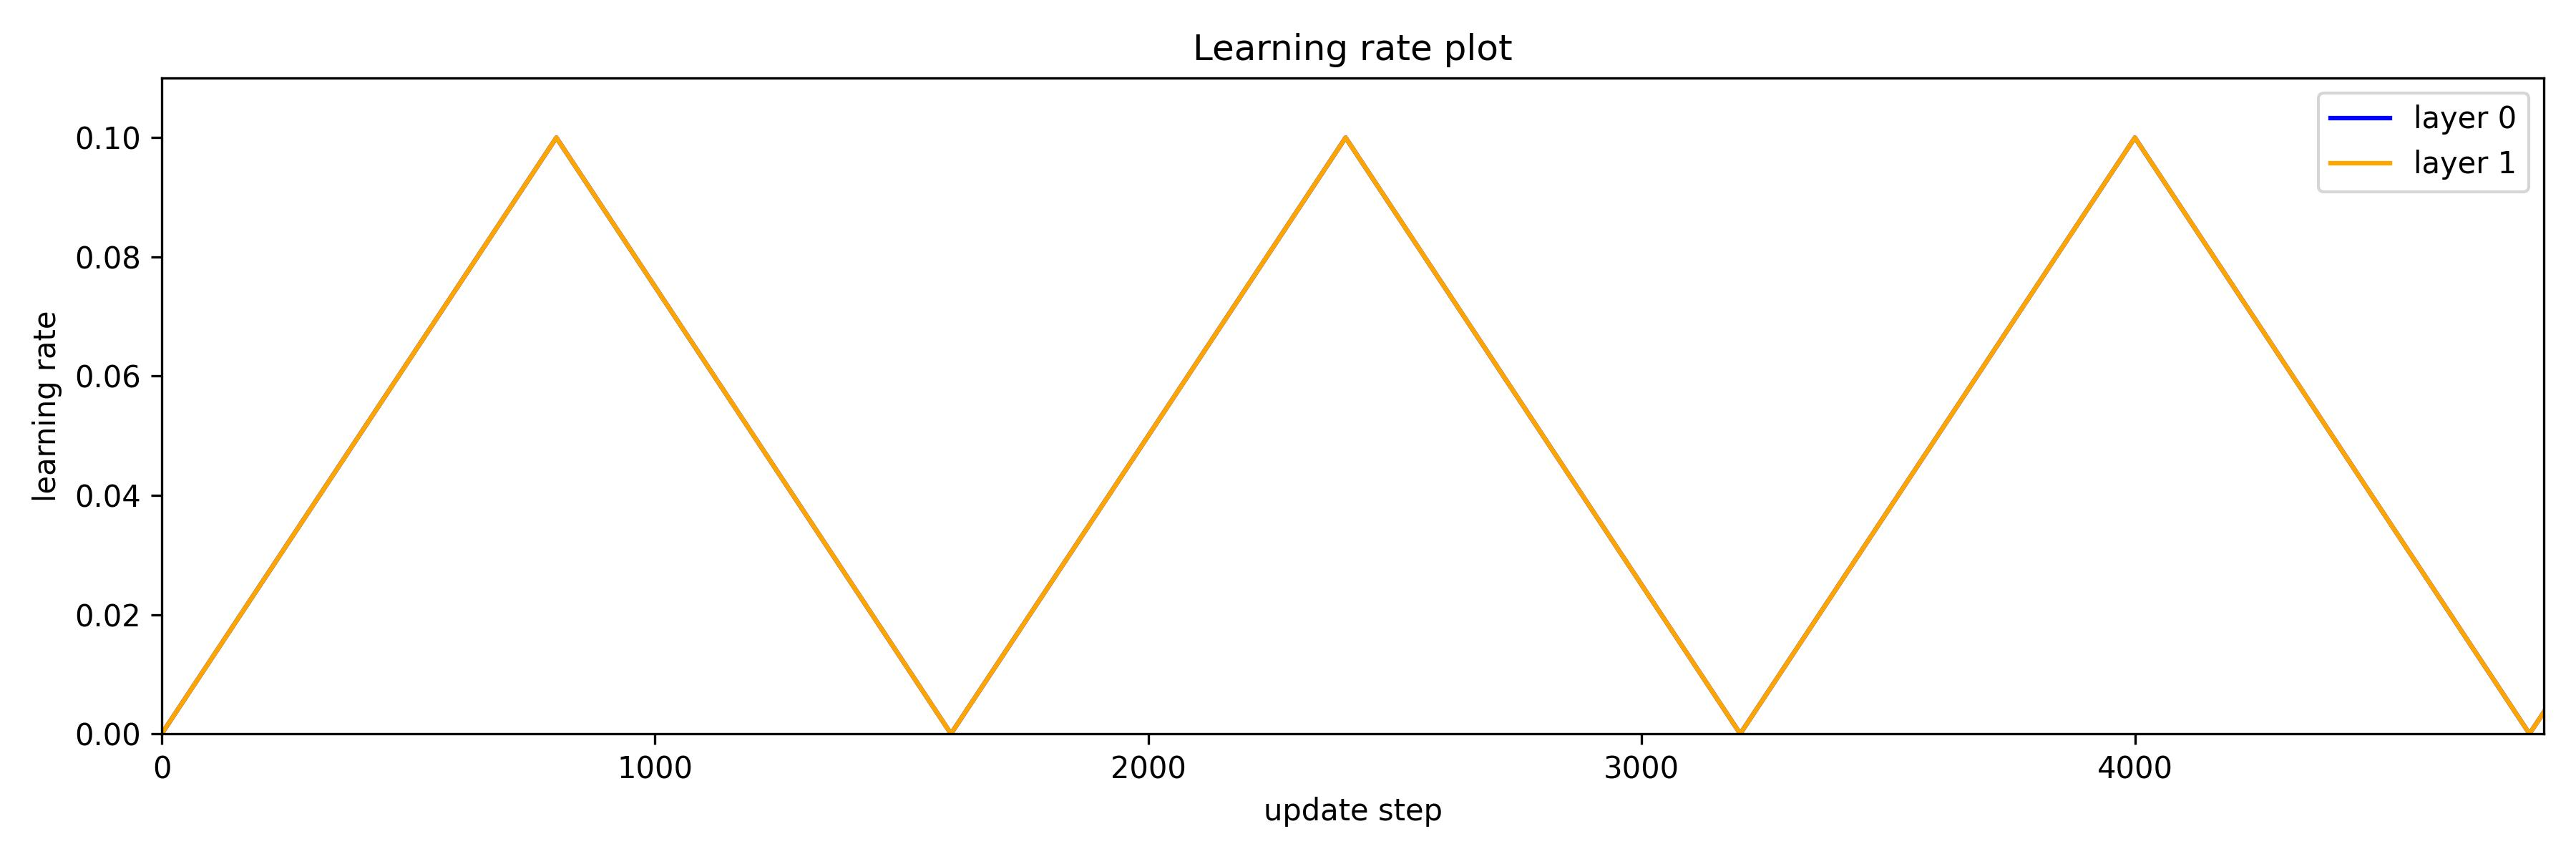
\includegraphics[width=0.8\textwidth]{cyclic_eta3.jpg}
    \caption{Plot of learning rate across the update steps with best lambda.}
    \label{fig:best_lambda_eta}
\end{figure}

The following are accuracy results:
\begin{lstlisting}[caption={Training and validation accuracy for best lambda}, label={lst:best_lambda_accuracy}]
Accuracy for training : 64.19% with steps 5880
Accuracy for validation : 54.70% with steps 5880
Accuracy for testing : 54.44% with steps 5880
\end{lstlisting}

The training curves for \( \lambda = 0.0022 \), identified through a coarse-to-fine grid search, show reduced overfitting and improved generalization compared to earlier experiments with \(\lambda = 0.01 \).
The training and validation losses are closer, and accuracy is more stable, indicating better regularization.



\end{document}